\documentclass{article}  % Add this line to specify the document class
\usepackage{natbib}      % For citation management
\usepackage{listings}
\usepackage{xcolor}
\usepackage{graphicx}
\usepackage{fancyhdr}    % For custom headers and footers
%\usepackage{amsmath}

% Define custom colors for better contrast
\definecolor{myblue}{rgb}{0.1, 0.2, 0.7}  % Darker blue
\definecolor{mygreen}{rgb}{0.0, 0.5, 0.2}  % Darker green
\definecolor{myred}{rgb}{0.7, 0.1, 0.1}  % Darker red
\definecolor{paleyellow}{rgb}{1.0, 1.0, 0.9}  % Very pale yellow for background

\pagestyle{fancy}
\fancyhf{}  % clear all headers and footers

% Make the header file monospace and smaller (optional)
\usepackage{fancyvrb}
\renewcommand{\headrulewidth}{0.4pt} % line under header

% Conditionally include header.txt
\IfFileExists{header.txt}{%
  \fancyhead[L]{% Auto-generated by make_header.sh
\usepackage{hyperref}
\newcommand{\commitsha}{\href{https://github.com/tschm/demopaper/commit/782d2bd8ddd430e1e311aeec805921e0dbcf8e89}{\texttt{782d2bd-dirty}}}
\newcommand{\branchname}{\texttt{main}}
\newcommand{\commitdate}{\texttt{2025-07-26}}
\newcommand{\reponame}{\href{https://github.com/tschm/demopaper}{\texttt{tschm/demopaper}}}
\newcommand{\tagname}{\href{https://github.com/tschm/demopaper/releases/tag/v0.5.0-dirty}{\texttt{v0.5.0-dirty}}}
}%
}{}

% Setup fancy headers
%\pagestyle{fancy}
%\fancyhf{} % Clear all header and footer fields
%\fancyhead[R]{\textcolor{blue}{% Auto-generated by make_header.sh
\usepackage{hyperref}
\newcommand{\commitsha}{\href{https://github.com/tschm/demopaper/commit/782d2bd8ddd430e1e311aeec805921e0dbcf8e89}{\texttt{782d2bd-dirty}}}
\newcommand{\branchname}{\texttt{main}}
\newcommand{\commitdate}{\texttt{2025-07-26}}
\newcommand{\reponame}{\href{https://github.com/tschm/demopaper}{\texttt{tschm/demopaper}}}
\newcommand{\tagname}{\href{https://github.com/tschm/demopaper/releases/tag/v0.5.0-dirty}{\texttt{v0.5.0-dirty}}}
{}{}}} % Add tag to the right header in blue
%%\fancyhead[R]{\textcolor{blue}{Hello World}}
%\renewcommand{\headrulewidth}{0pt} % Remove header rule

\lstset{
  language=Python,
  basicstyle=\ttfamily\small,
  keywordstyle=\color{myblue},       % Darker blue for keywords
  commentstyle=\color{mygreen},      % Darker green for comments
  stringstyle=\color{myred},         % Darker red for strings
  numbers=left,
  numberstyle=\tiny\color{gray},     % Use gray for line numbers
  frame=single,
  backgroundcolor=\color{paleyellow}, % Set very pale yellow background
  breaklines=true,
  showstringspaces=false
}

\title{A Brief Overview of the Simple Harmonic Oscillator}
\author{Peter Maffay}
\date{\today}

\begin{document}
\maketitle
%\thispagestyle{fancy}

\begin{abstract}
    Hello Tag: \InputIfFileExists{header.txt}{}{}
This paper provides a brief overview of the simple harmonic oscillator,
focusing on its mathematical description and physical significance. We discuss
the fundamental equation of motion and its solution, demonstrating why this
system serves as a cornerstone model in physics.
\end{abstract}

\section{Introduction}
The simple harmonic oscillator is one of the most fundamental models in physics.
Its applications range from the motion of pendulums to the behavior of atoms
in crystal lattices \citep{feynman1963}.

\section{Mathematical Description}
The equation of motion for a simple harmonic oscillator is given by:

\begin{equation}
    \frac{d^2x}{dt^2} + \omega^2x = 0
\end{equation}

where $\omega$ is the angular frequency of oscillation. The general solution
to this equation is:

\begin{equation}
    x(t) = A\cos(\omega t + \phi)
\end{equation}

where $A$ is the amplitude and $\phi$ is the phase constant
\citep{goldstein2002}.

\begin{lstlisting}
# Python code to calculate sum of squares of first 10 numbers
def sum_of_squares(n):
    return sum(i**2 for i in range(1, n+1))

result = sum_of_squares(10)
print(f"The sum of squares of first 10 numbers is: {result}")
\end{lstlisting}

\begin{figure}[h]
    \centering
    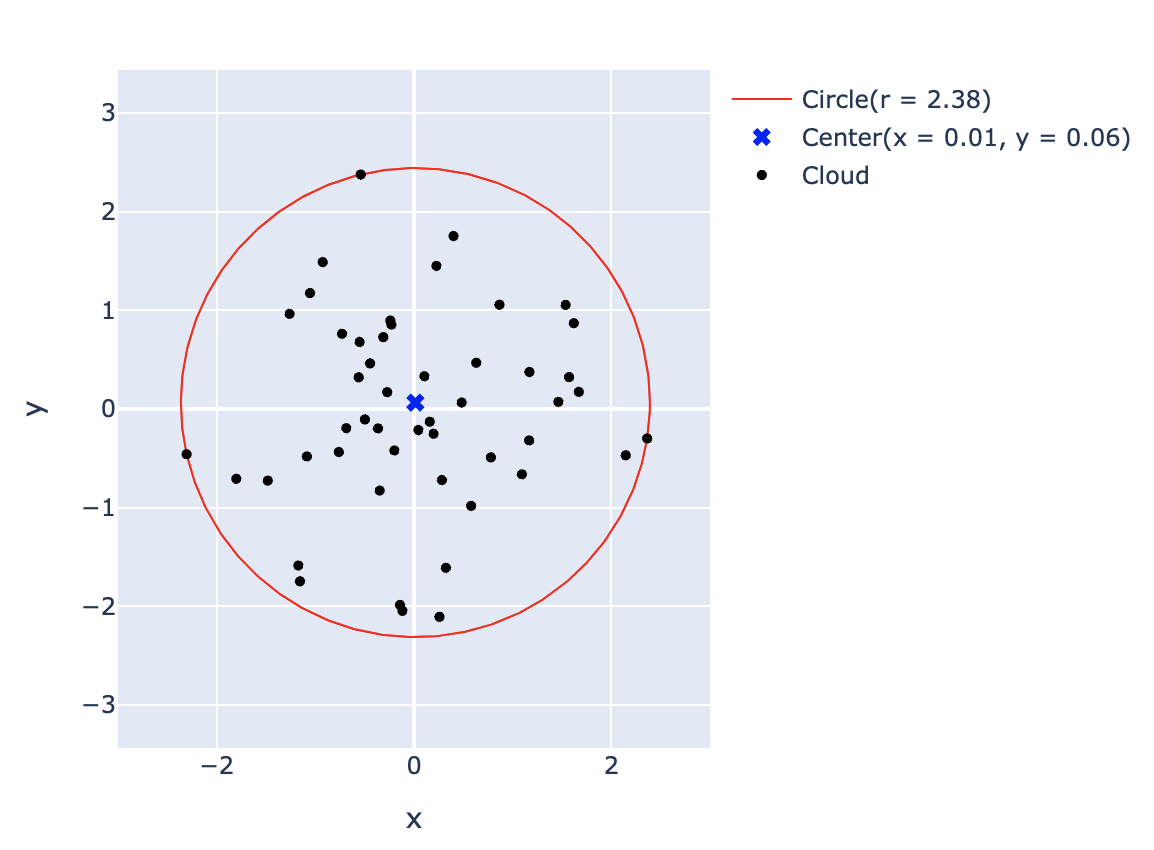
\includegraphics[width=0.8\textwidth]{graph.png} % Adjust width as needed
    \caption{This is an example image}
    \label{fig:example}
\end{figure}

\bibliography{references}
\bibliographystyle{plainnat}

\end{document}
